%%%%%%%%%%%%%%%%%%%%%%%%%
% PACKAGES              %
%%%%%%%%%%%%%%%%%%%%%%%%%
\documentclass[]{report} % book|article|…

\usepackage[utf8x]{inputenc}    % accents
\usepackage{geometry}           % marges
\usepackage[francais]{babel}    % langue
\usepackage{graphicx}           % images
\usepackage{verbatim}           % texte préformaté
\usepackage{fancyhdr}           % fancy
\usepackage{filecontents}       % write file directly
\usepackage{csvsimple}          % csv reader
\usepackage{lastpage}	        % get number of last page
\usepackage{listings}           % source code 
\usepackage{url}                % clickable urls 
\usepackage{float}              % exact placing of figures
\usepackage{amsmath}            % fancy matrices
\usepackage{xkeyval}            % keywords arguments for newcommand
\usepackage{xifthen}            % provides \isempty test

% packages for graphics
\usepackage{fancybox}         
\usepackage{pgfplots}        
\usepackage{pgfplotstable}
\usepgfplotslibrary{dateplot}
\usepackage{pgfplots}

\definecolor{Gene0}{RGB}{250, 164, 1}
\definecolor{Gene1}{RGB}{128, 0, 128}
\definecolor{Gene2}{RGB}{255, 0, 0}
\definecolor{Gene3}{RGB}{58, 242, 75}
\definecolor{Gene4}{RGB}{8, 81, 156}
\definecolor{Diversity}{RGB}{0, 0, 0}

\pgfplotscreateplotcyclelist{list}{
        {Gene0},
        {Gene1},
        {Gene2},
        {Gene3},
        {Gene4},
        {Diversity}
}




%%%%%%%%%%%%%%%%%%%%%%%%%
% SIMULATION COMMAND    %
%%%%%%%%%%%%%%%%%%%%%%%%%
%This is needed for encapsulating.
%changes the catcode of @ so it
%can be used freely (not needed
%when writing a package)
\makeatletter

\define@cmdkey [SIMPAR] {fam} {generations} [200] {}
\define@cmdkey [SIMPAR] {fam} {popsize}     [300] {}
\define@cmdkey [SIMPAR] {fam} {parents}     [2]   {}
\define@cmdkey [SIMPAR] {fam} {seed}        [4223]{}
\define@cmdkey [SIMPAR] {fam} {mutationrate}[0.0001] {}
\define@cmdkey [SIMPAR] {fam} {initialpheno}[1-11-11] {}
 
\presetkeys [SIMPAR] {fam} {generations = 1,
                            popsize = 2,
                            parents = 3,
                            seed = 4,
                            mutationrate = 5,
                            initialpheno = 6,
                           }{}

\newcommand{\simulationParameters}[1]{%
        \setkeys[SIMPAR]{fam}{#1}
        \begin{tabular}{|l|c||l|c|}
        \hline
        \textbf{Generations computed} & \cmdSIMPAR@fam@generations & \textbf{Population size}     & \cmdSIMPAR@fam@popsize \\ \hline
        \textbf{Parent number}        & \cmdSIMPAR@fam@parents     & \textbf{Seed}                & \cmdSIMPAR@fam@seed    \\ \hline
        \textbf{Mutation rate}        & \cmdSIMPAR@fam@mutationrate& \textbf{Initial Phenotype}   & \cmdSIMPAR@fam@initialpheno \\ \hline
        \end{tabular}
}

%Change again the @ catcode
%to normal
\makeatother




%%%%%%%%%%%%%%%%%%%%%%%%%
% PRÉAMBULE             %
%%%%%%%%%%%%%%%%%%%%%%%%%
\title{Genomat\\PRJ project Report}
\author{Ostiane D'AUGUSTIN and Lucas BOURNEUF}
% laisser vide pour date de compilation
\date{} 

% FORMAT PAGES         
\pagestyle{fancy} % nom du rendu (définit les lignes suivantes)
        \lhead{M1 BIG} % left head
        \chead{} % center head
        \rhead{2014/2015} % right head
        \lfoot{} % left foot
        \cfoot{\thepage/\pageref{LastPage}} % center foot
        \rfoot{} % right foot






%%%%%%%%%%%%%%%%%%%%%%%%%
% BEGIN                 %
%%%%%%%%%%%%%%%%%%%%%%%%%
\begin{document}
        \maketitle % page de titre




%%%%%%%%%%%%%%%%%%%%%%%%%
% SECTION               %
%%%%%%%%%%%%%%%%%%%%%%%%%
\section*{Introduction}
	\paragraph*{}
	The aim of this project is to implement a genetic algorithm which will bring out the connexions between different genes, 
        their regulation networks, and some properties linked to, as well as their resistance to genes knock-out (KO).
	\paragraph*{}
	We will study a famous genes network example, which has been highlighted by Wagner. Wagner's genes network is an artificial genes network calculation model. 
        It has explained all the development and evolution process of genetic regulation networks. It has been first developed by Andreas Wagner in 1996, 
        and then used by several research teams in order to study genes network evolution, genes expression, etc.
	\paragraph*{}
	We will simulate \textit{in silico} a population's evolution over many generations. Each individual is caracterized by his genotype 
        (that is to say, its genes network). 
        Individuals will be submit to an evolutive process by the intermediary of their genes networks.




%%%%%%%%%%%%%%%%%%%%%%%%%
% SECTION               %
%%%%%%%%%%%%%%%%%%%%%%%%%
\section*{Project organization}
	\paragraph*{}
        The project follows a Python-like packaging, with the main program launchable as a package. (\textit{python -m genomat})
        Many parameters can be sended through command-line arguments, or configuration file.
        Outputs are mainly in \textsc{csv format}. (notabily those provided for statistics)

	\paragraph*{}
        A second and incomplete implementation of Genomat is available under the name of \textit{genomat\_func}. 
        This implementation is only here as a proof of concept that use a functionnal approach.

	\paragraph*{}
        Used technologies :
        \begin{description}
                \item[python] as the main language (version 3.4);
                \item[docopt] as command-line arguments parser;
                \item[doctest] for unit tests in some docstrings (see \textsc{unittests.py} file);
                \item[numpy] for manage matrix (and notabily multiplications) until Python 3.5 interpreter is available;
                \item[latex] for present report, with pgfplot module for automatic data vizualization generation;
                \item[pylint] for source code profiling and UML generation;
                \item[make] for automatize simulations, tests, etc;
        \end{description}





%%%%%%%%%%%%%%%%%%%%%%%%%
% SECTION               %
%%%%%%%%%%%%%%%%%%%%%%%%%
\section*{Source code architecture}
	\paragraph*{}
        Genomat is cut in modules as shown in Figure~\ref{fig:umldiag}, and described below.
        \begin{description}
                \item[main] implements a simple and efficient interface that allow command-line arguments;
                \item[config] management of configurations : files, options, flags, serialization;
                \item[gene network] definition of an individual, encapsulation of numpy matrix system;
                \item[population] a list of individuals that provides many data access and call stats modules as an observer;
                \item[stats] observer of population that tests it and generate, if asked, data in targeted files;
                \item[progress bar] dumb and simple implementation of a progress bar, designed to be replaced later;
        \end{description}

        \begin{figure}[H] 
                \centering
                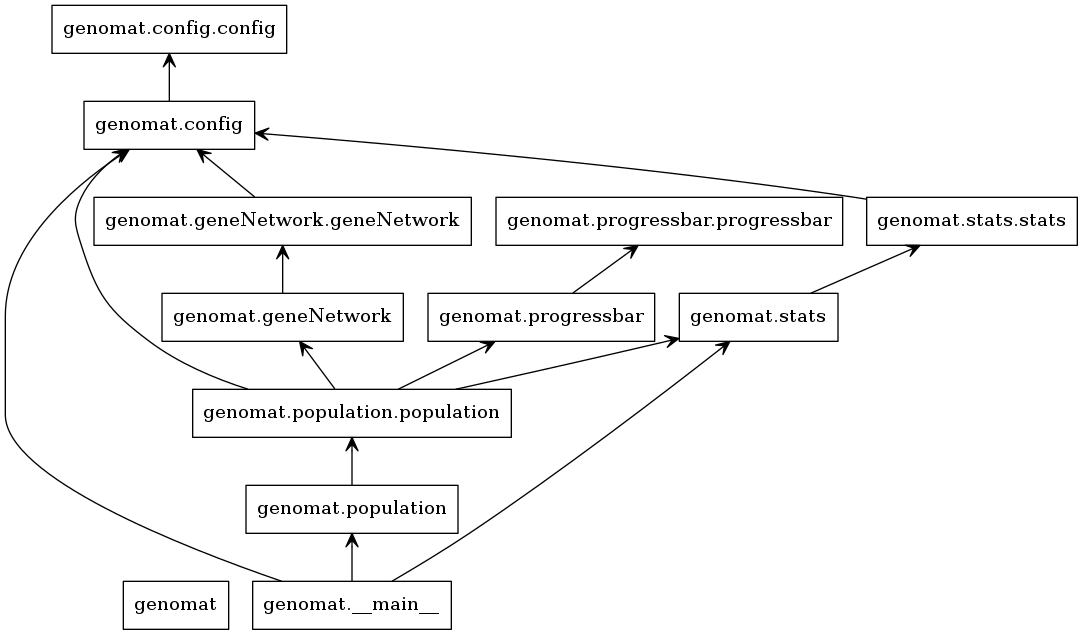
\includegraphics[width=\textwidth]{packages_genomat.png}
                \caption{\footnotesize Modules of Genomat architecture, without externals ones (numpy, docopt).}
                \label{fig:umldiag}
        \end{figure}




%%%%%%%%%%%%%%%%%%%%%%%%%
% SECTION               %
%%%%%%%%%%%%%%%%%%%%%%%%%
\section{Watchables}
    \paragraph*{}
    Main data generated results of gene KO, for each gene at each generation. 
    A diversity ratio is also computed at each generation.
    \paragraph*{}
     First, as there was no mutation rate given, exploited simulations use a mutation rate from $10^{-0}$ to $10^{-6}$, 
     with a constant population size of 300 individuals and 200 generations.\\
     For each gene, the survavibility ratio is computed. \\The survivability ratio is defined as $S_{g} = \frac{KO_g}{population_{size}}$ 
     with $KO_g$ as the number of individuals still viable after the KO of gene g.



%%%%%%%%%%%%%%%%%%%%%%%%%
% SECTION               %
%%%%%%%%%%%%%%%%%%%%%%%%%
\section*{Results through graphics}
\subsection{Telltale}
    \paragraph*{}
    The used telltale follows the next rules :\\
    \simulationParameters{}
    \begin{figure}[H] 
      \centering
      \begin{tikzpicture}
          \begin{axis}[
                  %,no mark % retract marks at point location
                  ,xlabel={Generations}
                  ,ylabel={Survivability ratio}
                  ,grid=major % grid on all axis
                  ,axis lines=left
                  ,ymajorgrids
                  ,legend style={legend pos=south west}
                  ,cycle list name=list
              ]
              \addplot table [col sep=comma,x=generationnumber,y=viabilityratio0] {ps300xg200xmr1-10-4.csv};
              \addplot table [col sep=comma,x=generationnumber,y=viabilityratio1] {ps300xg200xmr1-10-4.csv};
              \addplot table [col sep=comma,x=generationnumber,y=viabilityratio2] {ps300xg200xmr1-10-4.csv};
              \addplot table [col sep=comma,x=generationnumber,y=viabilityratio3] {ps300xg200xmr1-10-4.csv};
              \addplot table [col sep=comma,x=generationnumber,y=viabilityratio4] {ps300xg200xmr1-10-4.csv};
              \addplot[line width=1.0pt, mark=x] 
                       table [col sep=comma,x=generationnumber,y=diversity]       {ps300xg200xmr1-10-4.csv};
              \legend{Gene 0, Gene 1, Gene 2, Gene 3, Gene 4, Diversity}
          \end{axis}
      \end{tikzpicture}
      \caption{\footnotesize Resistance to gene KO survivability ratio, over 200 generations, with a population of 300 individuals and a mutation rate of $10^{-4}$, use as telltale}
      \label{fig:ps300xg200xmr1-10-4}
    \end{figure}
    \paragraph*{}
    We chose to use the mutation rate of $10^{-4}$ as the default parameter because it is a medium value, which can be a "natural" mutation rate, to which it will be easy to compare the other data.
    \paragraph*{}
    First we can notice that genes have rather the same conduct : their resistance to KO survivability ratio first increase and then stabilize about more or less 1. But, we can distinguish two different conducts in that global trend. In one hand, genes 1, 3, 4 and even later gene 2 reach a resistance to KO survivability ratio equals to 1. It means that those genes, even once KO, do not avoid the individual's survival. In the other hand, the gene 0 never reaches resistance to KO survivability ratio of 1. It approaches the 150th and the 160th generations, but does not reaches it for all that. It means that this gene 0 is more essential for the individual's survival.
    \paragraph*{}
    As a result, we can notice that the diversity is slowly decreasing during the 50 first generations. Then, it decreases rather fastly from 1 to 0.4 up to the 150th generation, where it finaly stabilizes around 0.35. Indeed, as there is only one gene to be essential, and as the mutation rate is pretty low, the global population phenotype is stabilizing, which lowers the diversity.

    \begin{figure}[H] 
            \centering
            \small
    $
            \begin{pmatrix}
                150 +- 190 & -2 +- 335 & 177 +- 295 & 23 +- 175 & 4 +- 1426 \\
                146 +- 10206 & 76 +- 9686 & -18 +- 4078 & 52 +- 9762 & -40 +- 2479 \\
                -4 +- 0 & -33 +- 401 & 208 +- 608 & -9 +- 85 & 42 +- 1103 \\
                -67 +- 4290 & -17 +- 472 & -56 +- 186 & 57 +- 1245 & 67 +- 3686 \\
                -7 +- 6196 & -53 +- 13893 & 33 +- 1259 & 2 +- 692 & 91 +- 1449 9 
            \end{pmatrix}
    $
            \caption{\footnotesize To look \& regenerate}
            \label{mat:ps300xg200xmr1-10-4}
    \end{figure}
    
    
    
    \subsection{Mutation rate variation}
    \paragraph*{}
    
    \paragraph*{}
    Parameters for the next experience :\\
    \simulationParameters{Mutation rate}
    \begin{figure}[H] 
      \centering
      \begin{tikzpicture}
          \begin{axis}[
                  %,no mark % retract marks at point location
                  ,xlabel={Generations}
                  ,ylabel={Survivability ratio}
                  ,grid=major % grid on all axis
                  ,axis lines=left
                  ,ymajorgrids
                  ,legend style={legend pos=south east}
                  ,cycle list name=list
              ]
              \addplot table [col sep=comma,x=generationnumber,y=viabilityratio0] {ps300xg200xmr1-10-0.csv};
              \addplot table [col sep=comma,x=generationnumber,y=viabilityratio1] {ps300xg200xmr1-10-0.csv};
              \addplot table [col sep=comma,x=generationnumber,y=viabilityratio2] {ps300xg200xmr1-10-0.csv};
              \addplot table [col sep=comma,x=generationnumber,y=viabilityratio3] {ps300xg200xmr1-10-0.csv};
              \addplot table [col sep=comma,x=generationnumber,y=viabilityratio4] {ps300xg200xmr1-10-0.csv};
              \addplot[line width=1.0pt, mark=x] 
                       table [col sep=comma,x=generationnumber,y=diversity]       {ps300xg200xmr1-10-0.csv};
              \legend{Gene 0, Gene 1, Gene 2, Gene 3, Gene 4, Diversity}
          \end{axis}
      \end{tikzpicture}
      \caption{\footnotesize Resistance to gene KO survivability ratio, over 200 generations, with a population of 300 individuals and a mutation rate of 1}
      \label{fig:ps300xg200xmr1-10-0}
    \end{figure}
    \paragraph*{}
    A mutation rate of 1 means that each gene of each individual of each generation will mutate. It is a theorical case, wich can not happen in a natural population.
    \paragraph*{}
    As each gene mutates, there is no resistance to gene KO survivability ratio stabilization, as we could see for the telltale. Each gene is more or less essential. We do not notice a stabilization to a resistance to gene KO survivability of 1, however, all the lines are beyond 0.9, which is very good. As each gene mutates, the diversity is very high (a constant equals to 1), and even if a gene is KO, the diversity given by the mutations allow the invidual to be viable.

    \begin{figure}[H] 
            \centering
            \small
    $
            \begin{pmatrix}
                304 +- 8526 & -39 +- 33750 & 119 +- 15040 & 15 +- 8066 & -26 +- 4692 \\
                138 +- 21689 & 291 +- 7052 & 94 +- 33661 & 55 +- 10078 & 62 +- 17995 \\
                326 +- 9222 & 121 +- 2688 & 156 +- 10334 & -90 +- 9970 & -234 +- 19612 \\
                87 +- 6326 & -78 +- 9487 & 63 +- 5292 & 223 +- 6283 & 128 +- 14690 \\
                15 +- 25929 & 58 +- 25518 & 2 +- 10437 & -80 +- 5527 & 241 +- 9406 
            \end{pmatrix}
    $
            \caption{\footnotesize To look \& regenerate}
            \label{mat:ps300xg200xmr1-10-0}
    \end{figure}
    
    
    \paragraph*{}
    Parameters for the next experience :\\
    \simulationParameters{Mutation rate}
    \begin{figure}[H] 
    \centering
    \begin{tikzpicture}
       \begin{axis}[
                  %,no mark % retract marks at point location
                  ,xlabel={Generations}
                  ,ylabel={Survivability ratio}
                  ,grid=major % grid on all axis
                  ,axis lines=left
                  ,ymajorgrids
                  ,legend style={legend pos=south east}
                  ,cycle list name=list
              ]
              \addplot table [col sep=comma,x=generationnumber,y=viabilityratio0] {ps300xg200xmr1-10-1.csv};
              \addplot table [col sep=comma,x=generationnumber,y=viabilityratio1] {ps300xg200xmr1-10-1.csv};
              \addplot table [col sep=comma,x=generationnumber,y=viabilityratio2] {ps300xg200xmr1-10-1.csv};
              \addplot table [col sep=comma,x=generationnumber,y=viabilityratio3] {ps300xg200xmr1-10-1.csv};
              \addplot table [col sep=comma,x=generationnumber,y=viabilityratio4] {ps300xg200xmr1-10-1.csv};
              \addplot[line width=1.0pt, mark=x] 
                       table [col sep=comma,x=generationnumber,y=diversity]       {ps300xg200xmr1-10-1.csv};
              \legend{Gene 0, Gene 1, Gene 2, Gene 3, Gene 4, Diversity}
          \end{axis}
      \end{tikzpicture}
      \caption{\footnotesize Resistance to gene KO survivability ratio, over 200 generations, with a population of 300 individuals and a mutation rate of $10^{-1}$}
      \label{fig:ps300xg200xmr1-10-1}
    \end{figure}
    \paragraph*{}
    A mutation rate of $10^{-1}$ is still very high for a natural population, and the global conduct is similar to the previous graph ones. However, the resistance to gene KO survivability ratios are lower than the previous. As the mutation rate is lower, there is a bit more phenotype stabilization, and thus, a gene can easier become essential. For example, it is the case of the gene 0, which waits for the 60th generation to become unessential and stabilize around 1; contrary to gene 1 which is first unessential, and becomes more and more essential as the time spends.
    \paragraph*{}
    Nevertheless, the diversity is still very high (constant equals to 1), which explains the pretty good resistance to gene KO survivability ratios.
   

    \begin{figure}[H] 
            \centering
            \small
    $
            \begin{pmatrix}
                98 +- 6039 & -26 +- 2711 & 28 +- 3244 & 75 +- 2903 & 13 +- 926 \\
                -39 +- 2815 & 152 +- 3468 & 45 +- 700 & -33 +- 796 & -45 +- 658 \\
                -31 +- 2053 & 71 +- 9285 & 120 +- 6335 & 9 +- 5160 & 80 +- 6374 \\
                -22 +- 4187 & -53 +- 612 & 27 +- 693 & 68 +- 785 & 152 +- 2428 \\
                39 +- 3960 & 47 +- 4600 & 14 +- 5258 & 2 +- 1785 & 116 +- 1672 
            \end{pmatrix}
    $
            \caption{\footnotesize To look \& regenerate}
            \label{mat:ps300xg200xmr1-10-1}
    \end{figure}
    
    
    \paragraph*{}
    Parameters for the next experience :\\
    \simulationParameters{Mutation rate}
    \begin{figure}[H] 
    \centering
    \begin{tikzpicture}
        \begin{axis}[
                  %,no mark % retract marks at point location
                  ,xlabel={Generations}
                  ,ylabel={Survivability ratio}
                  ,grid=major % grid on all axis
                  ,axis lines=left
                  ,ymajorgrids
                  ,legend style={legend pos=south east}
                  ,cycle list name=list
              ]
              \addplot table [col sep=comma,x=generationnumber,y=viabilityratio0] {ps300xg200xmr1-10-2.csv};
              \addplot table [col sep=comma,x=generationnumber,y=viabilityratio1] {ps300xg200xmr1-10-2.csv};
              \addplot table [col sep=comma,x=generationnumber,y=viabilityratio2] {ps300xg200xmr1-10-2.csv};
              \addplot table [col sep=comma,x=generationnumber,y=viabilityratio3] {ps300xg200xmr1-10-2.csv};
              \addplot table [col sep=comma,x=generationnumber,y=viabilityratio4] {ps300xg200xmr1-10-2.csv};
              \addplot[line width=1.0pt, mark=x] 
                       table [col sep=comma,x=generationnumber,y=diversity]       {ps300xg200xmr1-10-2.csv};
              \legend{Gene 0, Gene 1, Gene 2, Gene 3, Gene 4, Diversity}
          \end{axis}
      \end{tikzpicture}
      \caption{\footnotesize Resistance to gene KO survivability ratio, over 200 generations, with a population of 300 individuals and a mutation rate of $10^{-2}$}
      \label{fig:ps300xg200xmr1-10-2}
    \end{figure}
    \paragraph*{}
   

    \begin{figure}[H] 
            \centering
            \small
    $
            \begin{pmatrix}
                201 +- 5007 & -10 +- 3188 & 35 +- 8854 & -10 +- 7485 & 51 +- 666 \\
                55 +- 106 & 298 +- 215 & 61 +- 227 & 35 +- 100 & 80 +- 265 \\
                41 +- 743 & 119 +- 1950 & 109 +- 3238 & -132 +- 7931 & 54 +- 1729 \\
                -62 +- 567 & -39 +- 1281 & -16 +- 93 & 167 +- 4186 & -55 +- 613 \\
                -164 +- 10949 & -82 +- 2716 & 106 +- 1495 & -84 +- 12073 & 162 +- 5029  
            \end{pmatrix}
    $
            \caption{\footnotesize To look \& regenerate}
            \label{mat:ps300xg200xmr1-10-2}
    \end{figure}    
    
      
    \paragraph*{}
    Parameters for the next experience :\\
    \simulationParameters{Mutation rate}    
    \begin{figure}[H] 
    \centering
    \begin{tikzpicture}
        \begin{axis}[
                  %,no mark % retract marks at point location
                  ,xlabel={Generations}
                  ,ylabel={Survivability ratio}
                  ,grid=major % grid on all axis
                  ,axis lines=left
                  ,ymajorgrids
                  ,legend style={legend pos=south west}
                  ,cycle list name=list
              ]
              \addplot table [col sep=comma,x=generationnumber,y=viabilityratio0] {ps300xg200xmr1-10-5.csv};
              \addplot table [col sep=comma,x=generationnumber,y=viabilityratio1] {ps300xg200xmr1-10-5.csv};
              \addplot table [col sep=comma,x=generationnumber,y=viabilityratio2] {ps300xg200xmr1-10-5.csv};
              \addplot table [col sep=comma,x=generationnumber,y=viabilityratio3] {ps300xg200xmr1-10-5.csv};
              \addplot table [col sep=comma,x=generationnumber,y=viabilityratio4] {ps300xg200xmr1-10-5.csv};
              \addplot[line width=1.0pt, mark=x] 
                       table [col sep=comma,x=generationnumber,y=diversity]       {ps300xg200xmr1-10-5.csv};
              \legend{Gene 0, Gene 1, Gene 2, Gene 3, Gene 4, Diversity}
          \end{axis}
      \end{tikzpicture}
      \caption{\footnotesize Resistance to gene KO survivability ratio, over 200 generations, with a population of 300 individuals and a mutation rate of $10^{-5}$}
      \label{fig:ps300xg200xmr1-10-5}
    \end{figure}
    \paragraph*{}
   

    \begin{figure}[H] 
            \centering
            \small
    $
            \begin{pmatrix}
                  193 +- 211 & 43 +- 1393 & 24 +- 80 & -80 +- 570 & 7 +- 362 \\
                  92 +- 1732 & 155 +- 75 & 106 +- 7319 & 105 +- 8293 & -15 +- 1104 \\
                  24 +- 3515 & 17 +- 3064 & 107 +- 9182 & 14 +- 1100 & -17 +- 1364 \\
                  -100 +- 1215 & 185 +- 7793 & 84 +- 415 & 164 +- 582 & -91 +- 191 \\
                  29 +- 2611 & 92 +- 1664 & 2 +- 2128 & 39 +- 5680 & 151 +- 499 
            \end{pmatrix}
    $
            \caption{\footnotesize To look \& regenerate}
            \label{mat:ps300xg200xmr1-10-5}
    \end{figure}

    
    \paragraph*{}
    Parameters for the next experience :\\
    \simulationParameters{Mutation rate}
    \begin{figure}[H] 
    \centering
    \begin{tikzpicture}
        \begin{axis}[
                  %,no mark % retract marks at point location
                  ,xlabel={Generations}
                  ,ylabel={Survivability ratio}
                  ,grid=major % grid on all axis
                  ,axis lines=left
                  ,ymajorgrids
                  ,legend style={legend pos=south west}
                  ,cycle list name=list
              ]
              \addplot table [col sep=comma,x=generationnumber,y=viabilityratio0] {ps300xg200xmr1-10-6.csv};
              \addplot table [col sep=comma,x=generationnumber,y=viabilityratio1] {ps300xg200xmr1-10-6.csv};
              \addplot table [col sep=comma,x=generationnumber,y=viabilityratio2] {ps300xg200xmr1-10-6.csv};
              \addplot table [col sep=comma,x=generationnumber,y=viabilityratio3] {ps300xg200xmr1-10-6.csv};
              \addplot table [col sep=comma,x=generationnumber,y=viabilityratio4] {ps300xg200xmr1-10-6.csv};
              \addplot[line width=1.0pt, mark=x] 
                       table [col sep=comma,x=generationnumber,y=diversity]       {ps300xg200xmr1-10-6.csv};
              \legend{Gene 0, Gene 1, Gene 2, Gene 3, Gene 4, Diversity}
          \end{axis}
      \end{tikzpicture}
      \caption{\footnotesize Resistance to gene KO survivability ratio, over 200 generations, with a population of 300 individuals and a mutation rate of $10^{-6}$}
      \label{fig:ps300xg200xmr1-10-6}
    \end{figure}
    \paragraph*{}
   

    \begin{figure}[H] 
            \centering
            \small
    $
          \begin{pmatrix}
                183 +- 1857 & 18 +- 629 & 4 +- 2699 & -67 +- 3022 & 28 +- 1536 \\
                59 +- 893 & 163 +- 0 & -74 +- 519 & 0 +- 68 & 8 +- 35 \\
                24 +- 1280 & 49 +- 1121 & 120 +- 1129 & 63 +- 1735 & 9 +- 345 \\
                -71 +- 5017 & 52 +- 852 & 52 +- 66 & 96 +- 3062 & 37 +- 8393 \\
                -8 +- 1308 & -1 +- 2278 & 48 +- 456 & -71 +- 573 & 162 +- 101 
           \end{pmatrix}
    $
            \caption{\footnotesize To look \& regenerate}
            \label{mat:ps300xg200xmr1-10-6}
    \end{figure}

    \paragraph*{}
    Parameters for the next experience :\\
    \simulationParameters{Mutation rate}
    \begin{figure}[H] 
    \centering
    \begin{tikzpicture}
        \begin{axis}[
                  %,no mark % retract marks at point location
                  ,xlabel={Generations}
                  ,ylabel={Survivability ratio}
                  ,grid=major % grid on all axis
                  ,axis lines=left
                  ,ymajorgrids
                  ,legend style={legend pos=south west}
                  ,cycle list name=list
              ]
              \addplot table [col sep=comma,x=generationnumber,y=viabilityratio0] {ps300xg200xmr1-10-10.csv};
              \addplot table [col sep=comma,x=generationnumber,y=viabilityratio1] {ps300xg200xmr1-10-10.csv};
              \addplot table [col sep=comma,x=generationnumber,y=viabilityratio2] {ps300xg200xmr1-10-10.csv};
              \addplot table [col sep=comma,x=generationnumber,y=viabilityratio3] {ps300xg200xmr1-10-10.csv};
              \addplot table [col sep=comma,x=generationnumber,y=viabilityratio4] {ps300xg200xmr1-10-10.csv};
              \addplot[line width=1.0pt, mark=x] 
                       table [col sep=comma,x=generationnumber,y=diversity]       {ps300xg200xmr1-10-10.csv};
              \legend{Gene 0, Gene 1, Gene 2, Gene 3, Gene 4, Diversity}
          \end{axis}
      \end{tikzpicture}
      \caption{\footnotesize Resistance to gene KO survivability ratio, over 200 generations, with a population of 300 individuals and a mutation rate of $10^{-10}$}
      \label{fig:ps300xg200xmr1-10-10}
    \end{figure}
    \paragraph*{}
   

    \begin{figure}[H] 
            \centering
            \small
    $
          \begin{pmatrix}
                183 +- 1857 & 18 +- 629 & 4 +- 2699 & -67 +- 3022 & 28 +- 1536 \\
                50 +- 0 & 163 +- 0 & -82 +- 0 & 3 +- 0 & 7 +- 0 \\
                62 +- 1789 & 53 +- 513 & 64 +- 3193 & 45 +- 1050 & 7 +- 154 \\
                -71 +- 5017 & 52 +- 852 & 52 +- 66 & 96 +- 3062 & 37 +- 8393 \\
                -8 +- 1308 & -1 +- 2278 & 48 +- 456 & -71 +- 573 & 162 +- 101 
          \end{pmatrix}
    $
            \caption{\footnotesize To look \& regenerate}
            \label{mat:ps300xg200xmr1-10-10}
    \end{figure}
    
    
    \subsection{Parents number variation}
    \paragraph*{}
    Parameters for the next experience :\\
    \simulationParameters{Parent number}
    \begin{figure}[H] 
    \centering
        \begin{tikzpicture}
            \begin{axis}[
                  %,no mark % retract marks at point location
                  ,xlabel={Generations}
                  ,ylabel={Survivability ratio}
                  ,grid=major % grid on all axis
                  ,axis lines=left
                  ,ymajorgrids
                  ,legend style={legend pos=south west}
                  ,cycle list name=list
              ]
              \addplot table [col sep=comma,x=generationnumber,y=viabilityratio0] {ps300xg200xmr1-10-4xprt300.csv};
              \addplot table [col sep=comma,x=generationnumber,y=viabilityratio1] {ps300xg200xmr1-10-4xprt300.csv};
              \addplot table [col sep=comma,x=generationnumber,y=viabilityratio2] {ps300xg200xmr1-10-4xprt300.csv};
              \addplot table [col sep=comma,x=generationnumber,y=viabilityratio3] {ps300xg200xmr1-10-4xprt300.csv};
              \addplot table [col sep=comma,x=generationnumber,y=viabilityratio4] {ps300xg200xmr1-10-4xprt300.csv};
              \addplot[line width=1.0pt, mark=x] 
                       table [col sep=comma,x=generationnumber,y=diversity]       {ps300xg200xmr1-10-4xprt300.csv};
              \legend{Gene 0, Gene 1, Gene 2, Gene 3, Gene 4, Diversity}
          \end{axis}
      \end{tikzpicture}
      \caption{\footnotesize Resistance to gene KO survivability ratio, over 200 generations, with a population of 300 individuals, a mutation rate of $10^{-4}$, and a parents number equals to the population size}
      \label{fig:ps300xg200xmr1-10-4xprt300}
    \end{figure}
    \paragraph*{}
   

    \begin{figure}[H] 
            \centering
            \small
    $
          \begin{pmatrix}
                158 +- 33 & -54 +- 45 & -34 +- 156 & -34 +- 23 & 19 +- 7 \\
                43 +- 29703 & 119 +- 2324 & -2 +- 1960 & 38 +- 4162 & 108 +- 167 \\
                40 +- 986 & 31 +- 1520 & 84 +- 1048 & -49 +- 2087 & 60 +- 4 \\
                7 +- 1727 & -50 +- 933 & 17 +- 360 & 96 +- 1686 & 51 +- 2458 \\
                32 +- 346 & -63 +- 25 & 51 +- 505 & -48 +- 1748 & 145 +- 228 
           \end{pmatrix}
    $
            \caption{\footnotesize To look \& regenerate}
            \label{mat:ps300xg200xmr1-10-4xprt300}
    \end{figure}
    
    
    
    
    \subsection{Initial phenotype variation}
    \paragraph*{}
    Parameters for the next experience :\\
    \simulationParameters{Initial Phenotype}
    \begin{figure}[H] 
    \centering
        \begin{tikzpicture}
            \begin{axis}[
                  %,no mark % retract marks at point location
                  ,xlabel={Generations}
                  ,ylabel={Survivability ratio}
                  ,grid=major % grid on all axis
                  ,axis lines=left
                  ,ymajorgrids
                  ,legend style={legend pos=south west}
                  ,cycle list name=list
              ]
              \addplot table [col sep=comma,x=generationnumber,y=viabilityratio0] {ps300xg200xmr1-10-4xalt1.csv};
              \addplot table [col sep=comma,x=generationnumber,y=viabilityratio1] {ps300xg200xmr1-10-4xalt1.csv};
              \addplot table [col sep=comma,x=generationnumber,y=viabilityratio2] {ps300xg200xmr1-10-4xalt1.csv};
              \addplot table [col sep=comma,x=generationnumber,y=viabilityratio3] {ps300xg200xmr1-10-4xalt1.csv};
              \addplot table [col sep=comma,x=generationnumber,y=viabilityratio4] {ps300xg200xmr1-10-4xalt1.csv};
              \addplot[line width=1.0pt, mark=x] 
                       table [col sep=comma,x=generationnumber,y=diversity]       {ps300xg200xmr1-10-4xalt1.csv};
              \legend{Gene 0, Gene 1, Gene 2, Gene 3, Gene 4, Diversity}
          \end{axis}
      \end{tikzpicture}
      \caption{\footnotesize Resistance to gene KO survivability ratio, over 200 generations, with a population of 300 individuals, a mutation rate of $10^{-4}$, and an alternative initial phenotype(-1,1,-1,1,-1)}
      \label{fig:ps300xg200xmr1-10-4xalt1}
    \end{figure}
    \paragraph*{}
   

    \begin{figure}[H] 
            \centering
            \small
    $
          \begin{pmatrix}
                150 +- 190 & -2 +- 335 & 177 +- 295 & 23 +- 175 & 4 +- 1426 \\
                146 +- 10206 & 76 +- 9686 & -18 +- 4078 & 52 +- 9762 & -40 +- 2479 \\
                -4 +- 0 & -33 +- 401 & 208 +- 608 & -9 +- 85 & 42 +- 1103 \\
                -67 +- 4290 & -17 +- 472 & -56 +- 186 & 57 +- 1245 & 67 +- 3686 \\
                -7 +- 6196 & -53 +- 13893 & 33 +- 1259 & 2 +- 692 & 91 +- 1449 
           \end{pmatrix}
    $
            \caption{\footnotesize To look \& regenerate}
            \label{mat:ps300xg200xmr1-10-4xalt1}
    \end{figure}
    
    
    \paragraph*{}
    Parameters for the next experience :\\
    \simulationParameters{Initial Phenotype}
    \begin{figure}[H] 
    \centering
    \begin{tikzpicture}
            \begin{axis}[
                  %,no mark % retract marks at point location
                  ,xlabel={Generations}
                  ,ylabel={Survivability ratio}
                  ,grid=major % grid on all axis
                  ,axis lines=left
                  ,ymajorgrids
                  ,legend style={legend pos=south west}
                  ,cycle list name=list
              ]
              \addplot table [col sep=comma,x=generationnumber,y=viabilityratio0] {ps300xg200xmr1-10-4xalt2.csv};
              \addplot table [col sep=comma,x=generationnumber,y=viabilityratio1] {ps300xg200xmr1-10-4xalt2.csv};
              \addplot table [col sep=comma,x=generationnumber,y=viabilityratio2] {ps300xg200xmr1-10-4xalt2.csv};
              \addplot table [col sep=comma,x=generationnumber,y=viabilityratio3] {ps300xg200xmr1-10-4xalt2.csv};
              \addplot table [col sep=comma,x=generationnumber,y=viabilityratio4] {ps300xg200xmr1-10-4xalt2.csv};
              \addplot[line width=1.0pt, mark=x] 
                       table [col sep=comma,x=generationnumber,y=diversity]       {ps300xg200xmr1-10-4xalt2.csv};
              \legend{Gene 0, Gene 1, Gene 2, Gene 3, Gene 4, Diversity}
          \end{axis}
      \end{tikzpicture}
      \caption{\footnotesize Resistance to gene KO survivability ratio, over 200 generations, with a population of 300 individuals, a mutation rate of $10^{-4}$, and an alternative initial phenotype (1,-1,1,-1,1)}
      \label{fig:ps300xg200xmr1-10-4xalt2}
    \end{figure}
    \paragraph*{}
   

    \begin{figure}[H] 
            \centering
            \small
    $
          \begin{pmatrix}
                150 +- 190 & -2 +- 335 & 177 +- 295 & 23 +- 175 & 4 +- 1426 \\
                146 +- 10206 & 76 +- 9686 & -18 +- 4078 & 52 +- 9762 & -40 +- 2479 \\
                -4 +- 0 & -33 +- 401 & 208 +- 608 & -9 +- 85 & 42 +- 1103 \\
                -67 +- 4290 & -17 +- 472 & -56 +- 186 & 57 +- 1245 & 67 +- 3686 \\
                -7 +- 6196 & -53 +- 13893 & 33 +- 1259 & 2 +- 692 & 91 +- 1449 
           \end{pmatrix}
    $
            \caption{\footnotesize To look \& regenerate}
            \label{mat:ps300xg200xmr1-10-4xalt2}
    \end{figure}
    
    
    \subsection{Population size variation}
    \paragraph*{}
    Parameters for the next experience :\\
    \simulationParameters{Population size}
    \begin{figure}[H] 
    \centering
    \begin{tikzpicture}
            \begin{axis}[
                  %,no mark % retract marks at point location
                  ,xlabel={Generations}
                  ,ylabel={Survivability ratio}
                  ,grid=major % grid on all axis
                  ,axis lines=left
                  ,ymajorgrids
                  ,legend style={legend pos=north east}
                  ,cycle list name=list
              ]
              \addplot table [col sep=comma,x=generationnumber,y=viabilityratio0] {ps20xg200xmr1-10-4.csv};
              \addplot table [col sep=comma,x=generationnumber,y=viabilityratio1] {ps20xg200xmr1-10-4.csv};
              \addplot table [col sep=comma,x=generationnumber,y=viabilityratio2] {ps20xg200xmr1-10-4.csv};
              \addplot table [col sep=comma,x=generationnumber,y=viabilityratio3] {ps20xg200xmr1-10-4.csv};
              \addplot table [col sep=comma,x=generationnumber,y=viabilityratio4] {ps20xg200xmr1-10-4.csv};
              \addplot[line width=1.0pt, mark=x] 
                       table [col sep=comma,x=generationnumber,y=diversity]       {ps20xg200xmr1-10-4.csv};
              \legend{Gene 0, Gene 1, Gene 2, Gene 3, Gene 4, Diversity}
          \end{axis}
      \end{tikzpicture}
      \caption{\footnotesize Resistance to gene KO survivability ratio, over 200 generations, with a population of only 20 individuals and a mutation rate of $10^{-4}$}
      \label{fig:ps20xg200xmr1-10-4}
    \end{figure}
    \paragraph*{}
   

    \begin{figure}[H] 
            \centering
            \small
    $
          \begin{pmatrix}
                150 +- 190 & -2 +- 335 & 177 +- 295 & 23 +- 175 & 4 +- 1426 \\
                146 +- 10206 & 76 +- 9686 & -18 +- 4078 & 52 +- 9762 & -40 +- 2479 \\
                -4 +- 0 & -33 +- 401 & 208 +- 608 & -9 +- 85 & 42 +- 1103 \\
                -67 +- 4290 & -17 +- 472 & -56 +- 186 & 57 +- 1245 & 67 +- 3686 \\
                -7 +- 6196 & -53 +- 13893 & 33 +- 1259 & 2 +- 692 & 91 +- 1449 
           \end{pmatrix}
    $
            \caption{\footnotesize To look \& regenerate}
            \label{mat:ps20xg200xmr1-10-4}
    \end{figure}
    
    
    
    \subsection{population size and parent count variation  (consanguinity in little population)}
    \paragraph*{}
    Parameters for the next experience :\\
    \simulationParameters{Population size, Parent number}
    \begin{figure}[H] 
    \centering
    \begin{tikzpicture}
            \begin{axis}[
                  %,no mark % retract marks at point location
                  ,xlabel={Generations}
                  ,ylabel={Survivability ratio}
                  ,grid=major % grid on all axis
                  ,axis lines=left
                  ,ymajorgrids
                  ,legend style={legend pos=north east}
                  ,cycle list name=list
              ]
              \addplot table [col sep=comma,x=generationnumber,y=viabilityratio0] {ps20xg200xprt20xmr1-10-4.csv};
              \addplot table [col sep=comma,x=generationnumber,y=viabilityratio1] {ps20xg200xprt20xmr1-10-4.csv};
              \addplot table [col sep=comma,x=generationnumber,y=viabilityratio2] {ps20xg200xprt20xmr1-10-4.csv};
              \addplot table [col sep=comma,x=generationnumber,y=viabilityratio3] {ps20xg200xprt20xmr1-10-4.csv};
              \addplot table [col sep=comma,x=generationnumber,y=viabilityratio4] {ps20xg200xprt20xmr1-10-4.csv};
              \addplot[line width=1.0pt, mark=x] 
                       table [col sep=comma,x=generationnumber,y=diversity]       {ps20xg200xprt20xmr1-10-4.csv};
              \legend{Gene 0, Gene 1, Gene 2, Gene 3, Gene 4, Diversity}
          \end{axis}
      \end{tikzpicture}
      \caption{\footnotesize Resistance to gene KO survivability ratio, over 200 generations, with a population of only 20 individuals and a mutation rate of $10^{-4}$}
      \label{fig:ps20xg200xprt20xmr1-10-4}
    \end{figure}
    \paragraph*{}
   

    \begin{figure}[H] 
            \centering
            \small
    $
          \begin{pmatrix}
                78 +- 0 & 40 +- 0 & -15 +- 0 & 56 +- 0 & 126 +- 0 \\
                136 +- 0 & 231 +- 0 & -3 +- 0 & 21 +- 0 & -40 +- 0 \\
                21 +- 0 & 153 +- 0 & 83 +- 0 & -6 +- 0 & -43 +- 0 \\
                -140 +- 0 & 75 +- 0 & 62 +- 0 & 126 +- 0 & 119 +- 0 \\
                72 +- 0 & 27 +- 0 & 156 +- 0 & -65 +- 0 & 162 +- 0 
           \end{pmatrix}
    $
            \caption{\footnotesize To look \& regenerate}
            \label{mat:ps20xg200xprt20xmr1-10-4}
    \end{figure}

%%%%%%%%%%%%%%%%%%%%%%%%%
% SECTION               %
%%%%%%%%%%%%%%%%%%%%%%%%%
%%%%%%%%%%%%%%%%%%%%%%%%%
% APPENDICES            %
%%%%%%%%%%%%%%%%%%%%%%%%%
%\newpage
%\begin{appendix}
%\section*{Annexes}

%\begin{figure}[h] % place it THERE (add ! for exact placement)
        %\centering
        %\pgfplotstabletypeset[
            %columns={time,wtf,error},
            %col sep=comma,
            %string type,
            %every head row/.style={%
                %before row={\hline
                    %& \multicolumn{2}{c}{useless data} \\
                    %},
                %after row=\hline
            %},
            %every last row/.style={after row=\hline},
            %columns/time/.style={column name=Time, column type=l},
            %columns/error/.style={column name=Primary key, column type=r},
            %columns/wtf/.style={column name=Concentration, column type=r},
        %]{data.csv}
        %\caption{Cool things that will be very useful for someone}
        %\label{ftab:cool}
%\end{figure}      



%\end{appendix}
\end{document}
% END
